%
% Master thesis template for Ghent University (2018)
%
%
%  !!!!!!!!!!!!!!!!!!!!!!!!!!!!!!!!!!!!!!!!!!!!!!!!!!!!!!!!!!!!
%  !!  MAKE SURE TO SET lualatex OR xelatex AS LATEX ENGINE  !!
%  !!!!!!!!!!!!!!!!!!!!!!!!!!!!!!!!!!!!!!!!!!!!!!!!!!!!!!!!!!!!
%  !! For overleaf:                                          !!
%  !!     1. click gear icon in top right                    !!
%  !!     2. select `lualatex` in "latex engine"             !!
%  !!     3. click "save project settings"                   !!
%  !!                                                        !!
%  !!!!!!!!!!!!!!!!!!!!!!!!!!!!!!!!!!!!!!!!!!!!!!!!!!!!!!!!!!!!
%
%
%  History
%    2014         Doctoral Thesis of Bruno Volckaert
%    2017         Adapted to master thesis by Jerico Moeyersons
%    2018         Cleanup by Merlijn Sebrechts
%
%  Latest version
%    https://github.com/galgalesh/masterproef-template
%
\documentclass[11pt,a4paper,twoside, openany]{book}
\usepackage[a4paper,includeheadfoot,margin=2.50cm]{geometry}

\setlength{\parindent}{0cm}           % indent of the first sentence of a paragraph
\setlength{\parskip}{1em}             % space between paragraphs
\renewcommand{\baselinestretch}{1.2}  % stretch horizontal space between everything

\usepackage{graphicx}
\graphicspath{{images/}}
\usepackage{pdfpages}
\usepackage{enumitem}
\usepackage{float}
\usepackage{caption}
\usepackage{subcaption}
\usepackage[toc,page]{appendix}

\usepackage{minted}                                    % for modern code highlighting
\newenvironment{code}{\captionsetup{type=listing}}{}   % To get multiline code fragments working: https://tex.stackexchange.com/a/53540/72273

\PassOptionsToPackage{hyphens}{url}
\usepackage{hyperref}
\usepackage{url}

\usepackage{quotchap}              % For the fancy quotes next to the chapter titles

\usepackage[numbers]{natbib}       % For bibliography; use numeric citations
\bibliographystyle{IEEEtran}
\usepackage[nottoc]{tocbibind}     % Put Bibliography in ToC

%
% Defines \checkmark to draw a checkmark
%
\usepackage{tikz}
\def\checkmark{\tikz\fill[scale=0.4](0,.35) -- (.25,0) -- (1,.7) -- (.25,.15) -- cycle;}

%
% For tables
%
\usepackage{booktabs}
\usepackage{array}
\usepackage{ragged2e}  % for '\RaggedRight' macro (allows hyphenation)
\newcolumntype{L}[1]{>{\raggedright\let\newline\\\arraybackslash\hspace{0pt}}m{#1}}
\newcolumntype{C}[1]{>{\centering\let\newline\\\arraybackslash\hspace{0pt}}m{#1}}
\newcolumntype{R}[1]{>{\raggedleft\let\newline\\\arraybackslash\hspace{0pt}}m{#1}}

%
% Support for splitting Dutch words correctly
%
\usepackage{polyglossia}
\setdefaultlanguage[babelshorthands=true]{dutch}

% Manually specify additional hypnations for words
\hyphenation{}

%
% Translated strings. If these aren't set, the English words are used.
%
\addto\captionsenglish{%
  \renewcommand{\contentsname}%
    {Inhoudsopgave}%
}
\renewcommand\appendixtocname{Bijlagen}
\renewcommand\appendixpagename{Bijlagen}
\renewcommand{\listoflistingscaption}{Lijst van listings}

\newfloat{code}{thp}{lop}
\floatname{code}{Code}

\newcommand\foreign[1]{\emph{#1}}
\newcommand\inlinecode[1]{\emph{#1}}
%
% Set the title and your name
%
\title{The user perceived performance of route planning APIs}
\author{Bert Marcelis}

%
%  END OF HEADER
%  The actual latex document content starts here.
%
\begin{document}

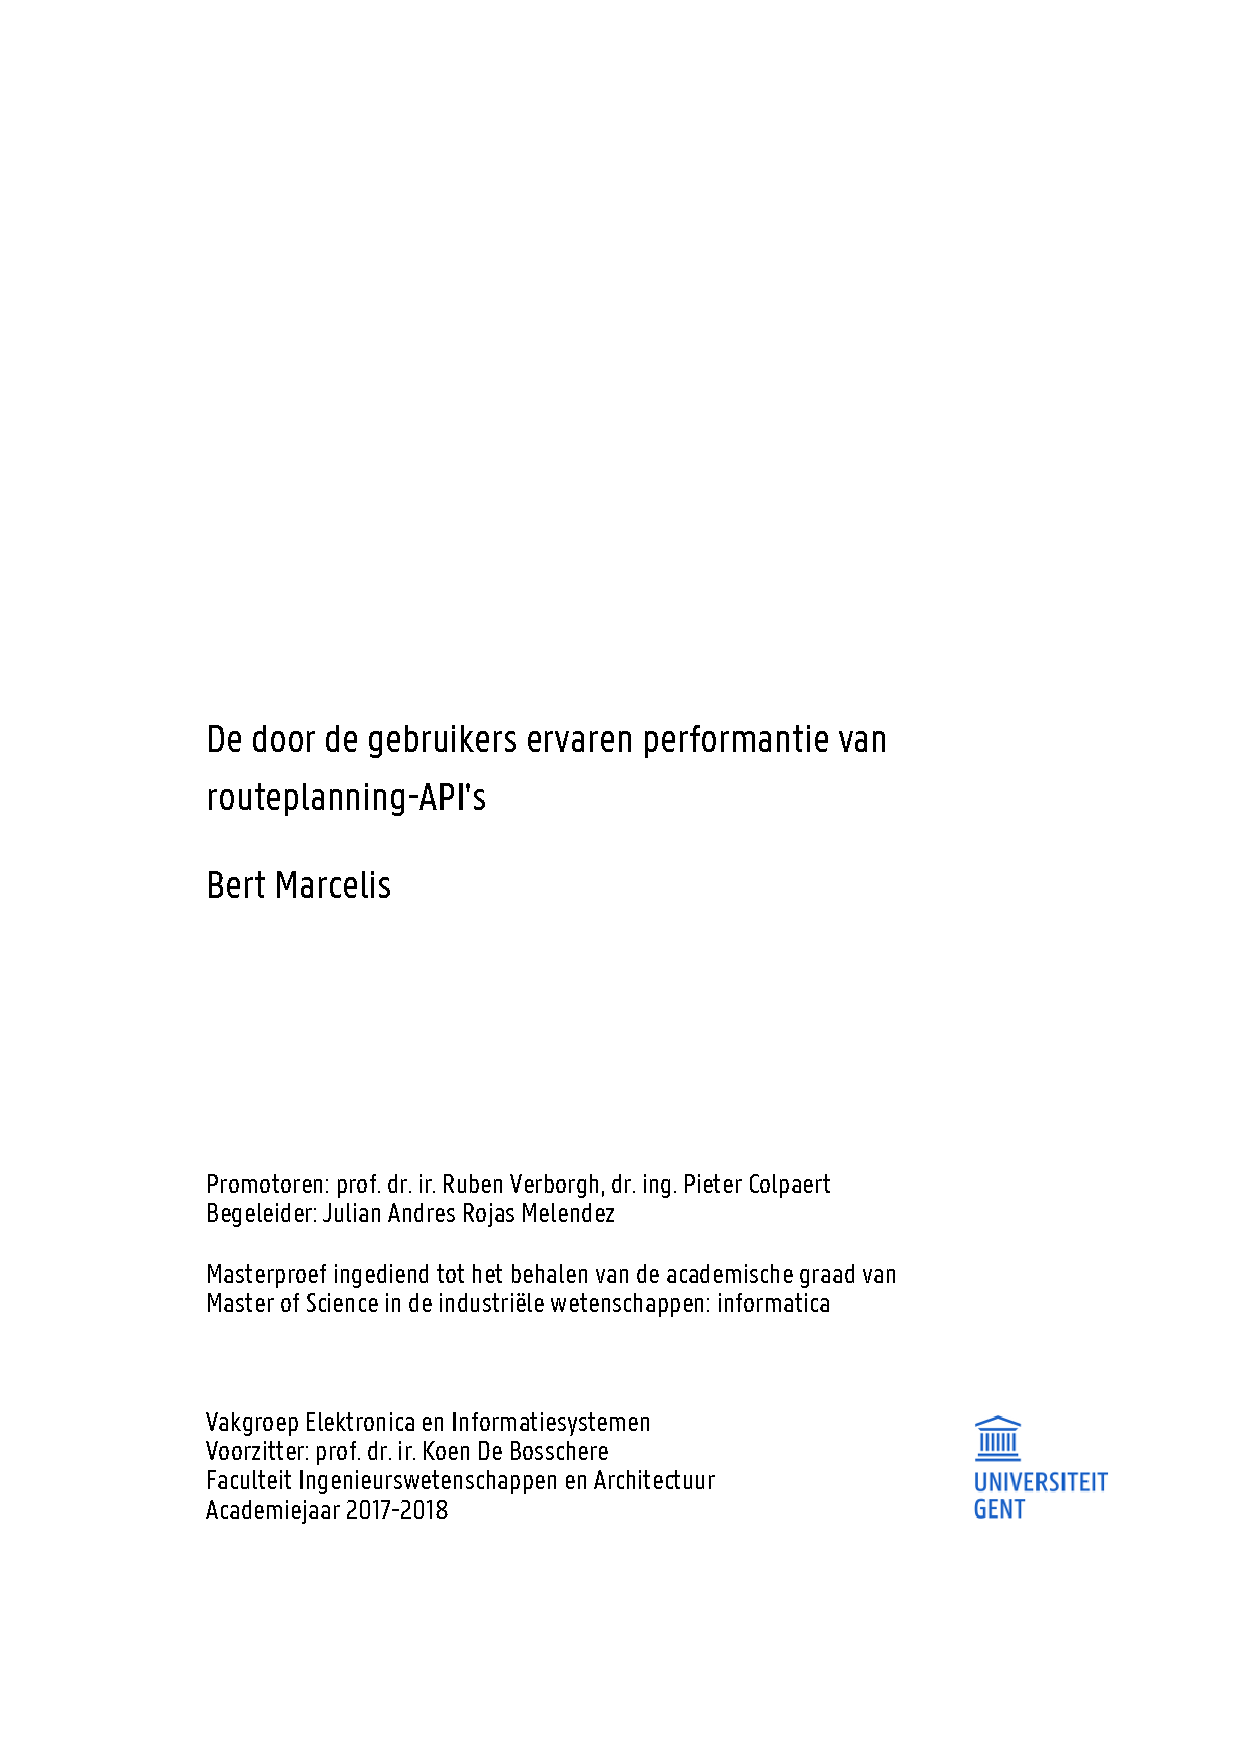
\includepdf{voorblad.pdf}             % Front matter
\newpage\thispagestyle{empty}\mbox{}  % White page
% !TeX spellcheck = nl_NL
\thispagestyle{empty}    % Don't show page number
\begin{center}
\textbf{Dankwoord}
\end{center}

Na zes maanden zwoegen is deze masterproef eindelijk klaar. Hoewel ik dit werk zelf moest maken, zou dit niet mogelijk geweest zijn zonder de hulp van een aantal mensen rondom mij. 

Als eerste wil ik mijn promotor Pieter Colpaert bedanken. Pieter, zonder jouw continue begeleiding, feedback, en talloze uren aan nalezen zou ik dit werk nooit tot een goed einde hebben gebracht. Ik wil ook mijn begeleider Julian Melendez bedanken, voor de hulp bij het verder ontwikkelen van Linked Connections en het nalezen van mijn scriptie.

Daarnaast wil ik ook graag mijn ouders bedanken, voor de steun en om altijd klaar te staan als ik hulp nodig had en te zorgen dat ik na een week hard werken steeds in een warm nest kon thuiskomen. Ik wil ook mijn vriendin Sofie bedanken voor de steun, de aanmoediging en het geduld doorheen deze maanden van hard werk. Ook mijn vrienden wil ik hier niet vergeten, die steeds voor wat ontspanning konden zorgen tussen de schrijf- of werksessies in.

Tot slot wens ik iedereen te bedanken die heeft bijgedragen aan het onderzoek, door deel te nemen aan de user-testing, door de enquête in te vullen, of door mee te helpen bij het verspreiden van de enquête.

Bedankt iedereen!

Bert Marcelis
          % Word of thanks
\newpage\thispagestyle{empty}\mbox{}  % White page
%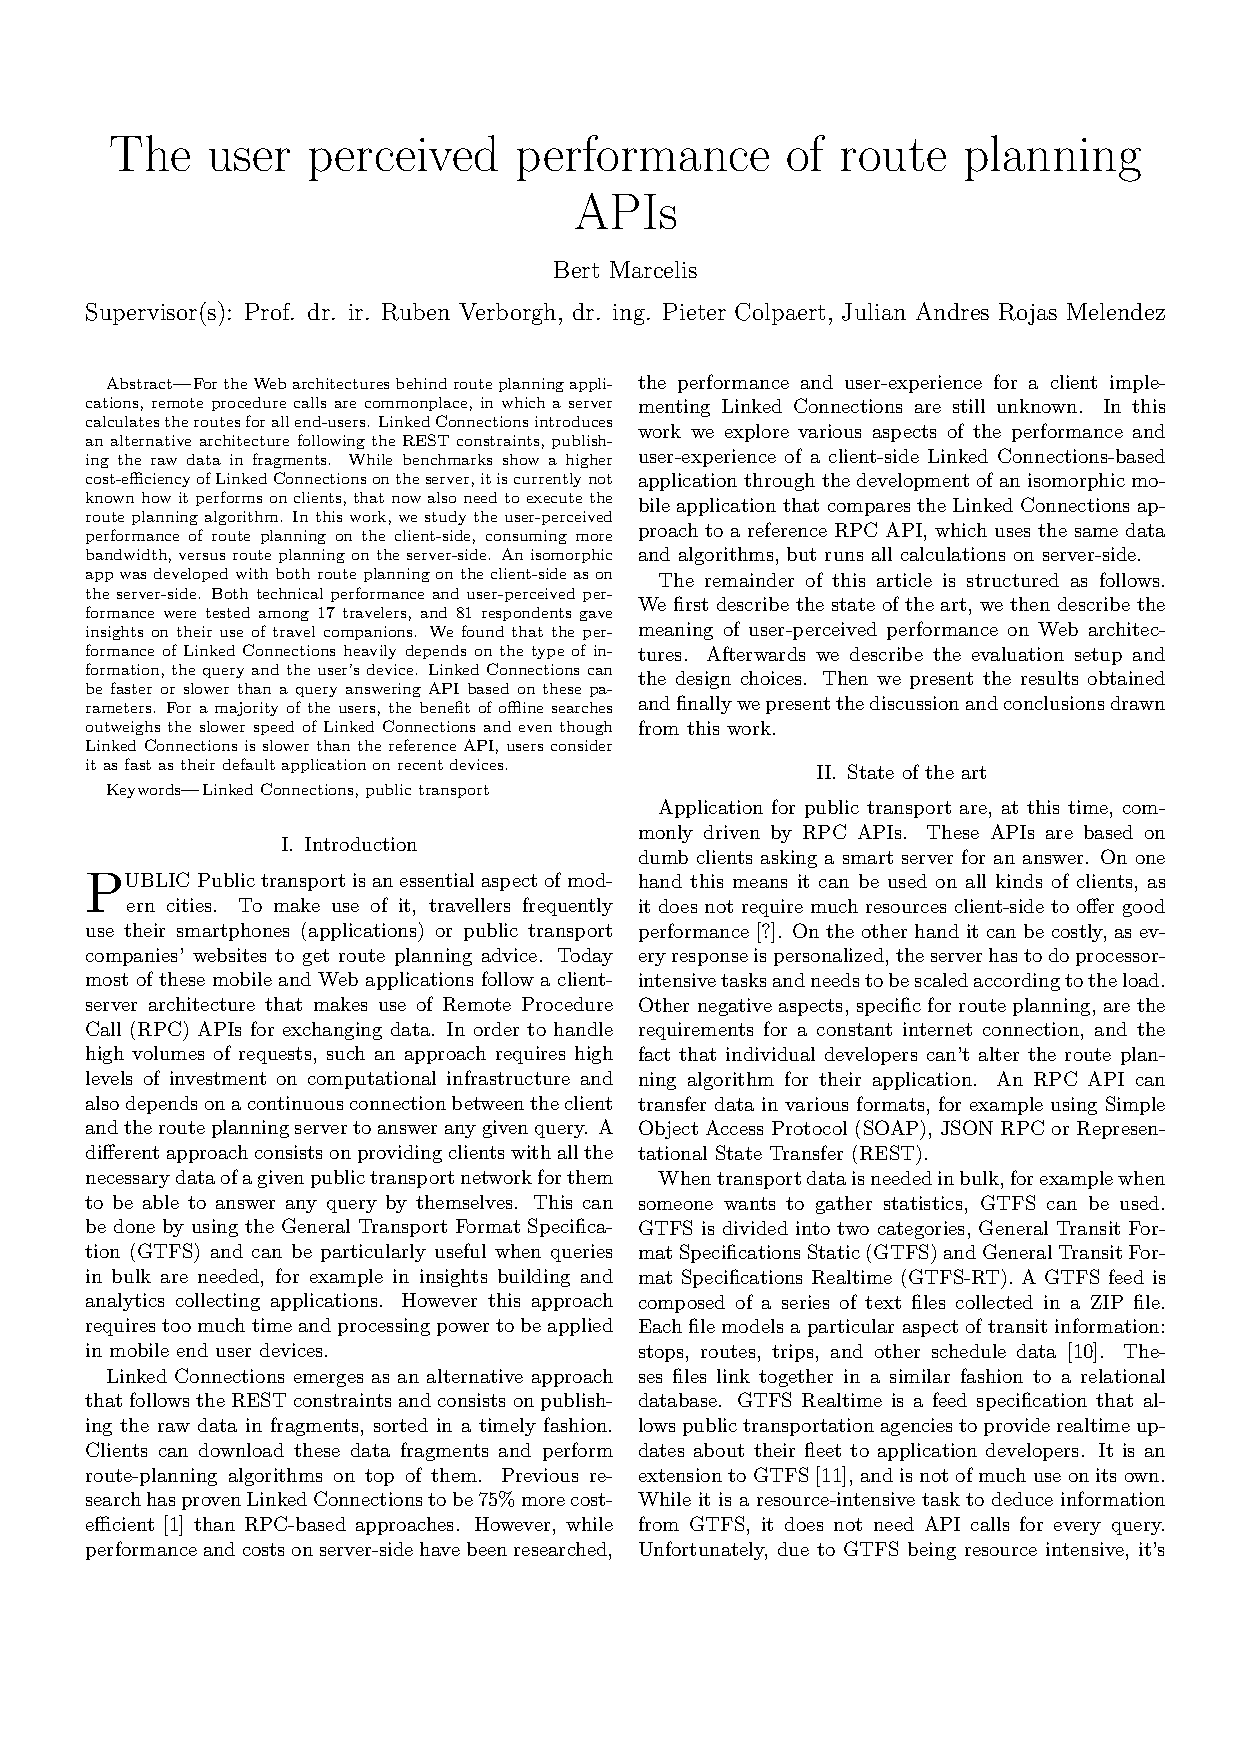
\includepdf[pages={-}]{abstract.pdf}  % Extended Abstract
\tableofcontents                      % Table of Contents
\listoffigures                        % List of figures
\listoftables                         % List of tables
\listoflistings                       % List of listings (code fragments)

%
% Include the main chapters of the thesis below
%
\begin{savequote}[0.55\linewidth]
	``Inspirational quote''
	\qauthor{\textasciitilde Source}
\end{savequote}

\chapter{Inleiding}
\label{chap:intro}
Openbaar vervoer is ook een essentiële dienst in elke stad\citep{programmableweb14}. Om vlot van dit openbaar vervoer gebruik te maken, zijn er tientallen websites en apps (user-agents) die gebruikers informatie verstrekken over vertrekken, aankomsten, ritten, routes en vertragingen. Voorbeelden hiervan in België zijn iRail.be, HyperRail en Railer, en CityMapper, TheTransitApp, Here WeGo en Google maps wereldwijd. Op dit moment zijn al deze user-agents echter toegewezen op het gebruik van data dumps of specifieke APIs om informatie met betrekking tot openbaar vervoer te publiceren, of een variant ervan. 

Enerzijds zijn er volledige data dumps, in de vorm van General Transit Feed Specification (GTFS)\footnote{https://developers.google.com/transit/gtfs/} en General Transit Feed Specification Realtime (GTFS-RT)\footnote{https://developers.google.com/transit/gtfs-realtime/}. GTFS bestanden bevatten informatie over alle voertuigen van een dienstverlener, over een relatief grote tijdspanne, typisch enkele maanden tot een jaar. GTFS-RT bestanden bevatten realtime informatie over ritten in de komende dag. Om al deze data compact op te slaan en te versturen, worden deze opgeslagen in de vorm van regels. Deze regels omschrijven wanneer welk voertuig welke rit maakt. Om op basis van deze regels vragen te beantwoorden, dient deze set abstracte regels omgevormd te worden naar een gepast model waarin ritten en stopplaatsen opgevraagd kunnen worden, en routes berekend kunnen worden. Hiervoor zijn, afhankelijk van welke informatie gewenst is, zware berekeningen vereist, die afhankelijk van de grootte van het GTFS bestand vijf à tien minuten kunnen duren op een moderne computer. Gebruikers kunnen geen 10 minuten wachten tot de data getransformeerd zijn, waardoor deze optie niet beschikbaar is op mobiele toestellen. Verder is dit formaat een mogelijke technologische restrictie op de vervoersdata: enkel gevorderde ontwikkelaars kunnen hiervan gebruik maken. Open data is slechts open als deze (onder andere) beschikbaar zijn in een begrijpbaar formaat~\citep{okfn18}. GTFS is dus vooral geschikt om vervoersdata te delen met grote bedrijven, en in mindere mate voor individuele ontwikkelaars die vervoers data eenvoudig willen visualiseren (digital signage, routeplanner applicaties, websites, ...).

\begin{figure}
	\centering
	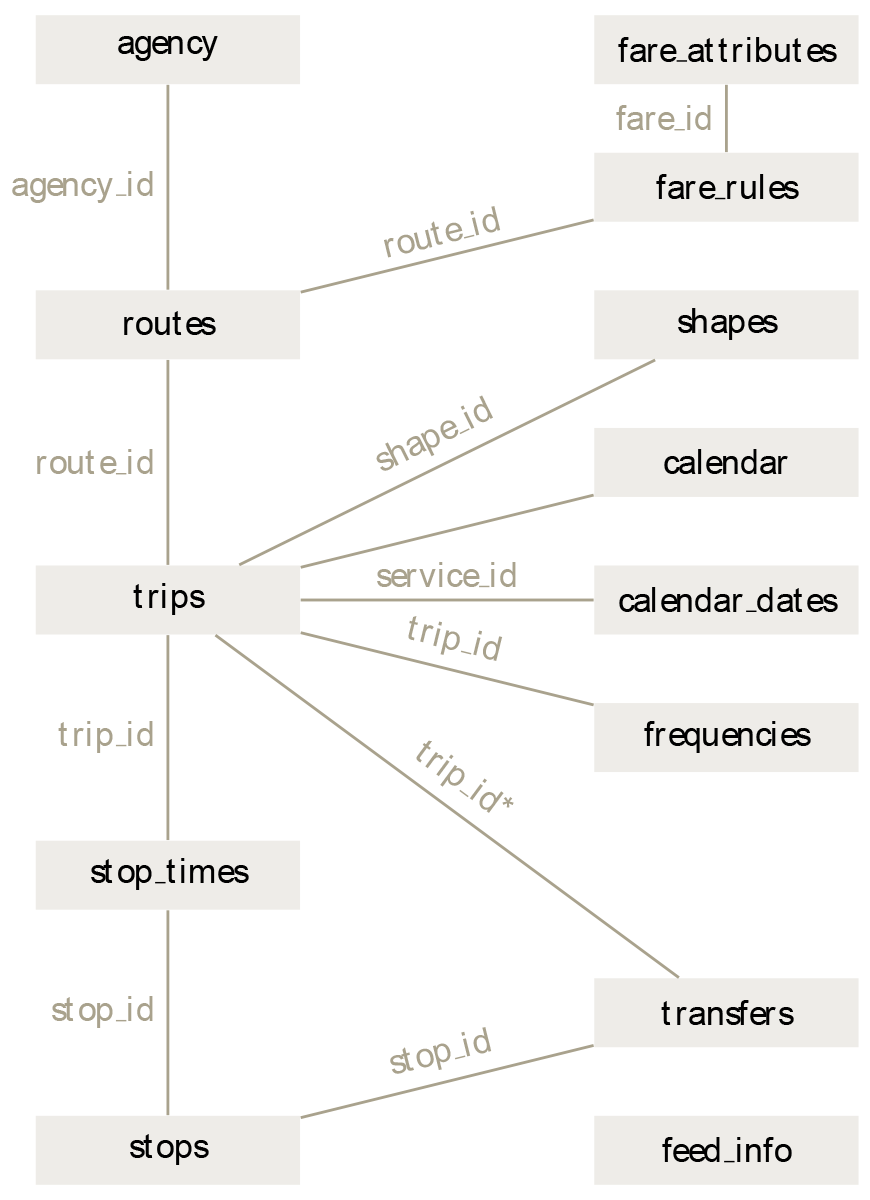
\includegraphics[width=0.5\textwidth]{GTFS_class_diagram.png}
		\caption[GTFS structuur]{De bestandsstructuur van GTFS data.}
	\label{fig:ldfAxis}
\end{figure}
% TODO: visueler maken wat GTFS juist is
 
Anderzijds zijn er traditionele Remote Procedure Call (RPC) zoals iRail\footnote{https://irail.be}, die beschikken over verschillende endpoints die specifieke vragen kunnen beantwoorden. Achterliggend kunnen zware berekeningen uitvoeren of grote databases raadplegen zonder dat de gebruiker hier nadeel van ondervindt. Deze antwoorden zijn rechtstreeks bruikbaar voor de client toepassing, maar bieden enkel een antwoord op één specifieke vraag. Een andere vraag, al dan niet door dezelfde client, vereist een nieuwe request naar de server, en zal een ander antwoord tot gevolg hebben. Elk verzoek naar de server vraagt relatief veel processortijd langs de serverkant. Een continue internetverbinding is dus vereist, en server-side is een potentieel grote en dure infrastructuur nodig om aan alle vragen te voldoen. Een ander belangrijk nadeel bij deze techniek is dat deze data moeilijk te combineren zijn met andere datasets. Een route plannen die gebruik maakt van meerdere openbaar vervoer aanbieders is enkel mogelijk als iemand een API aanbiedt die achterliggend door meerdere datasets zoekt. Simpelweg twee API's combineren is niet mogelijk.

\begin{figure}
	\centering
	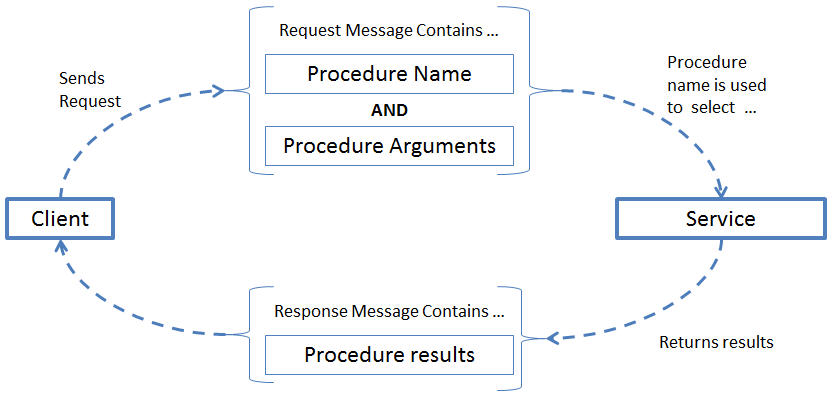
\includegraphics[width=0.80\textwidth]{RPC_API.jpg}
	\caption[RPC structuur]{De werkwijze van een RPC API.}
	\label{fig:ldfAxis}
\end{figure}

Deze twee methodes zijn elkaars tegengestelde. Ontwikkelaars moeten kiezen voor data die compact maar complex, en slechts indirect bruikbaar is, of voor een vraag-antwoord systeem wat voor elke nieuwe vraag een nieuw verzoek naar een server moet maken. Aan de IDLab onderzoeksgroep aan UGent is onderzoek gedaan naar Linked Connections (LC)\footnote{https://linkedconnections.org}, een nieuw formaat dat een nieuw evenwicht tracht te vinden. Alle vertrekken van alle voertuigen worden in één chronologische lijst verzameld, waarbij de lijst kan opgevraagd worden volgens vaste tijdsintervallen met een grootteorde van enkele minuten. Hierdoor hoeft de server enkel deze lijst in fragmenten aan te bieden, waarbij alle clients dezelfde informatie krijgen. De clients dienen zelf nog berekeningen te maken, maar deze zijn relatief eenvoudig vergeleken met de berekeningen die nodig zijn om een GTFS feed te verwerken. Data in het Linked Connections formaat kunnen eenvoudig toegankelijk gemaakt worden via een open-source serverapplicatie\footnote{https://github.com/julianrojas87/linked-connections-server/}.

\begin{figure}
	\centering
		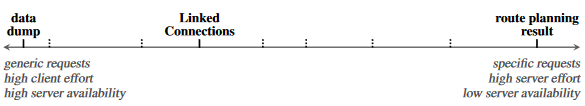
\includegraphics[width=0.80\textwidth]{ldfAxis.png}
	\caption[Routeplanning HTTP interfaces op de LDF as]{De Linked Data Fragments as illustreert dat alle HTTP interfaces data fragmenten aanbieden, maar verschillen in hoe specifiek de aangeboden data is, en dus de moeilijkheid om deze aan te maken~\citep{verborgh14}. In deze figuur is de as toegepast op HTTP interfaces voor routeplanning~\citep{colpaert15}.}
	\label{fig:ldfAxis}
\end{figure}

\section{Wat is user-perceived performance?}
\label{sec:what_is_user_perceived_performance}
Elke interface voor het ophalen van data heeft specifieke eigenschappen zoals latency, performance, cache hergebruik,~...~\citep{verborgh16}. Wanneer we verschillende technieken vergelijken door dezelfde user-agent, kunnen we de impact van de verschillende achterliggende technieken op de eindgebruiker onderzoeken. Hiervoor definiëren we de user-perceived performance. De user-perceived performance is de performance zoals de gebruiker deze ervaart, welke niet strikt gelijk hoeft te zijn aan de performance van technische component. De user-perceived latency werd gedefinieerd in 2000 door Roy T. Fielding gedefinieerd als de tijd tussen het selecteren van een link en het renderen van een bruikbaar resultaat~\citep{fielding99}. Latency treedt op op verschillende punten: 
\begin{enumerate}
	\item de tijd die de client nodig heeft om actie te ondernemen 
	\item de tijd die nodig is voor voorbereidende acties
	\item de tijd om een verzoek te verzenden
	\item de tijd die de server nodig heeft om te antwoorden
	\item de tijd die nodig is om het antwoord te verzenden
	\item de tijd voor het antwoord te verwerken en weer te geven
\end{enumerate}
Terwijl enkel stappen 3, 4 en 5 rechtstreeks afhankelijk zijn van het netwerk, kunnen al deze stappen beïnvloed worden door de gebruikte techniek \citep{fielding99}.

Ondertussen zijn we geëvolueerd naar een wereld waarin data vaak mobiel geconsumeerd worden: 78\% van de Vlamingen beschikt over een smartphone, 80,5\% beschikt over een laptop. Slechts 41,8\% beschikt over een desktop-computer~\citep{digimeter17}. Hierbij zijn er ook andere aspecten die meespelen in de user experience: batterijgebruik en offline toegang tot data vormen een aanzienlijke factor in de user experience. Een applicatie presteert beter wanneer deze dezelfde data kan weergeven met aanzienlijk minder energieverbruik, of wanneer deze consistent goed presteert, ook wanneer netwerk slecht of niet beschikbaar is. Hoewel de user-perceived performance nog steeds gedomineerd wordt door de tijd tussen het selecteren van een link en het renderen van een bruikbaar resultaat, dienen we dus ook deze andere aspecten in rekening te brengen. Mobiele gebruikers hebben ook nog steeds angst om te veel data te verbruiken~\citep{ammelrooy17}.

% TODO: zal dit zo blijven of is er een trend ivm angst over datalimiet?

\section{Probleemstelling en doel van de masterproef}
\label{sec:problem}

Linked Connections werd ontwikkeld met de bedoeling een evenwicht te vinden tussen data dumps en RPC API's. In plaats van elke query op een server te beantwoorden, wordt een gelinkte lijst van connecties gepubliceerd. Linked Connections laat hierdoor toe om queries te beantwoorden door middel van een lineair groeiende lijst van connecties~\citep{colpaert15}. Bovendien gebruiken alle user-agents dezelfde lijst, waardoor deze zeer cachebaar is. Bij stijgende belasting daalt de tijd die nodig is per verzoek \citep{colpaert17}.

Terwijl de cost-efficiency van Linked Connections reeds is aangetoond, waarbij Linked Connections hetzelfde aantal verzoeken kan beantwoorden met slechts 25\% van de rekencapacteit\citep{colpaert17,Melendez17}, is er nog geen onderzoek gebeurt naar de user-perceived performance van een user-agent wanneer deze gebruik maakt van Linked Connections, vergeleken met wanneer deze zelfde user-agent gebruik maakt van een traditionele RPC API. 

In deze studie richten we ons specifiek op routeplanning gebruik makend van mobiele toestellen. Deze toestellen hebben minder processorkracht en geheugen vergeleken met traditionele computers, maar ook bandbreedte en beschikbaarheid van internet zijn vaak beperkt. In het slechtste geval is er geen netwerkverbinding, waarbij enkel een cache beschikbaar is. Verder zullen we ons specifiek richten op het verschil tussen een RPC REST API gebaseerd op Linked Connections~\citep{colpaert17} en de originele Linked Connections webserver. Als user-agent zullen we een fork van de Android HyperRail\footnote{https://hyperrail.be} applicatie gebruiken, gemodificeerd om de genoemde API's te gebruiken. Door deze testopstelling zijn de oorspronkelijke data, de server hardware, de user-agent en de client hardware gelijk bij elke vergelijking. Enkel het formaat voor serverinteracties en transport van data zal verschillen.

Om routes te berekenen zullen we gebruik maken van het Connection Scan Algorithm (CSA)~\citep{strasser13,strasser14,strasser17}. Dit algoritme vereist een op vertrektijd gesorteerde lijst van vertrekken. Dit is de exacte definitie van de LinkedConnections knowledge graph, waardoor dit algoritme zonder al te veel modificaties toegepast kan worden. Fragmenten kunnen hierbij geladen worden op het moment dat ze nodig zijn. We zullen dezelfde implementatie gebruiken zowel bij de client-side API als bij de server-side API om zo correct mogelijke resultaten te behalen. 

In eerste instantie zal een traditionele (RPC) API geschreven worden welke gebruik maakt van de Linked Connections fragmenten op de Solid State Disk (SSD) van de server. Deze API zal endpoints bevatten voor het tonen van vertrekken en aankomsten per station, het berekenen van routes, en voor het weergeven van het traject per trein. 
Vervolgens zal een API zonder specifieke server-side geïmplementeerd worden in de applicatie. Deze zal dezelfde informatie ter beschikking stellen in de applicatie, maar zal hiervoor enkel (delen van) de gelinkte lijst met vertrekken downloaden. 

Eenmaal beide API's volledig geïmplementeerd zijn, zal de user-experienced performance onderzocht worden. Hiertoe worden begeleide user tests gehouden, waarbij een aantal testgebruikers afwisselend met beide API's hun dagelijkse opzoekingen zullen uitvoeren, waarna ze aan de hand van een vragenlijst bevraagd zullen worden naar hun ervaringen en voorkeuren. Het is essentieel om de subjectieve ervaringen van gebruikers te bevragen, gezien verschillende gebruikers mogelijk verschillende afwegingen maken. We verwachten dat sommige gebruikers offline toegang waardevol zullen vinden, terwijl anderen mogelijk geen belang hechten aan offline toegang. Ook zal er technische data verzameld worden, zoals geheugen- en processorgebruik, laadtijden, en batterijverbruik. 

Deze masterproef zal gebruik maken van data afkomstig van de NMBS om routeplanning en realtime data over treinen in België weer te geven. Door de bron van de data te vervangen kan dit onderzoek ook toegepast worden op andere openbaar vervoer maatschappijen die gebruik maken van tijdsschema's, ongeacht het soort voertuig dat gebruikt wordt.

\section{Onderzoeksvraag}
 
 \paragraph{Hypothese 1} De gebruiker ervaart de mogelijkheid voor offline zoekopdrachten als een meerwaarde.
 
 \paragraph{Hypothese 2} De gebruiker ervaart de mogelijkheid om voorkeuren voor routes in te stellen (overstaptijd, toegankelijkheid, ...) als een meerwaarde.
 
 \paragraph{Onderzoeksvraag} Verbetert de user experience en user perceived perforance van een applicatie voor openbaar vervoer wanneer gebruik gemaakt wordt van Linked Connections in plaats van traditionele RPC API's?
\begin{savequote}[0.55\linewidth]
	``Inspirational quote''
	\qauthor{\textasciitilde Source}
\end{savequote}

\chapter{Implementatie}
Om een zo eerlijk mogelijke vergelijking te bekomen, zullen we zowel bij de client-side API als de server-side API dezelfde algorithmes toepassen. Gezien de jonge leeftijd van het Linked Connections framework zijn er nog geen algoritmes beschikbaar om deze data te verwerken. We zullen de ontwikkeling van deze algoritmen bespreken, met speciale aandacht voor het routeplanning algoritme vanwege de hogere complexiteit en de uitgebreide mogelijkheden.

\section{Linked Connections formaat}

In plaats van een dump van planningsdata of een volledige routeplanner te publiceren, publiceert Linked Connections paren van vertrek en aankomst voor elke treinrit, telkens van een station tot het volgende. Deze paren worden gesorteerd volgens vertrektijd. Hierna wordt deze lijst van paren gesplitst, om pagina's van gelijke grootte of gelijke tijdsduur te bekomen. Deze fragmenten kunnen gepubliceerd worden via HTTP als \foreign{JSON-LD}\footnote{https://json-ld.org/}, waarbij user-agents kunnen kiezen welke pagina's ze opvragen. Links in de gepubliceerde documenten zorgen ervoor dat user-agents steeds weten welke pagina ze als volgende moeten laden \citep{linkedconnections18}.

Om bovenstaande methode in de praktijk om te zetten, wordt gebruik gemaakt van de open source LC-Server\footnote{https://github.com/julianrojas87/linked-connections-server/}. Om GTFS om te zetten naar Linked Connections, wordt er achterliggend gebruik gemaakt van de gtfs2lc tool\footnote{https://github.com/linkedconnections/gtfs2lc}.

Deze data zijn publiek toegankelijk via https://graph.irail.be/.

\subsection{Vraag- en antwoordformaat}
Om een pagina met data op te halen, wordt een verzoek gemaakt naar de API, waarbij de vervoersmaatschappij en het gewenste tijdstip in ISO8601 formaat in de URL opgenomen worden.  Codefragment \ref{code:linkedconnections-response} toont een ingekort resultaat voor de vertrekken bij de NMBS op 20 maart 2018, 12:30. De volledige specificatie kan teruggevonden worden op de LC website\footnote{https://linkedconnections.org/specification/1-0}.

Verzoek: \inlinecode{https://graph.irail.be/sncb/connections?departureTime=2018-03-20T12:30:00.000Z}

Een voorbeeld van een LC pagina zien we in fragment \ref{code:2:linkedconnections-response}, met volgende data:
\begin{enumerate}
	\item \foreign{@context}: Deze lijst definieert de gebruikte namespaces en velden
	\item \foreign{hydra:next} en  \foreign{hydra:previous}: Links naar de pagina met respectievelijk de volgende en de voorgaande data
	\item \foreign{hydra:search}: Informatie over de huidige pagina
	\item \foreign{@graph}: Deze lijst bevat de eigenlijke data. Elk vertrek bevat de volgende informatie:
	\begin{enumerate}
			\item \foreign{departureStop}: De URI welke het station van vertrek uniek identificeert.
			\item \foreign{arrivalStop}: De URI welke het station van aankomst uniek identificeert.	\item departureTime, arrivalTime: De geplande tijden, respectievelijk bij vertrek en aankomst.
			\item \foreign{departureDelay}, \foreign{arrivalDelay}: De vertraging, respectievelijk bij vertrek en aakomst.
			\item \foreign{direction}: De richting van dit voertuig, wat vaak ook op de lichtkrant van het voertuig weergegeven wordt.
			\item \foreign{gtfs:trip}: Een URI welk de rit van het voertuig uniek identificeert
			\item \foreign{gtfs:route}: Een URI welk de route van het voertuig uniek identificeert
			\item \foreign{gtfs:pickupType} en \foreign{gtfs:dropOffType}: geeft aan of reizigers al dan niet kunnen op- of afstappen bij respectievelijk vertrek en aankomst
	\end{enumerate}
\end{enumerate}

\begin{code}
	\begin{minted}[breaklines,tabsize=2]{json}
		
		{
			"@context": {
			 "xsd": "http://www.w3.org/2001/XMLSchema#",
			"lc": "http://semweb.mmlab.be/ns/linkedconnections#",
			"hydra": "http://www.w3.org/ns/hydra/core#",
			"gtfs": "http://vocab.gtfs.org/terms#",
			"Connection": "lc:Connection",
			"...": "..."
			},
			"@id": "https://graph.irail.be/sncb/connections?departureTime=2018-03-20T12:30:00.000Z",
			"@type": "hydra:PagedCollection",
			"hydra:next": "https://graph.irail.be/sncb/connections?departureTime=2018-03-20T12:40:00.000Z",
			"hydra:previous": "https://graph.irail.be/sncb/connections?departureTime=2018-03-20T12:20:00.000Z",
			"hydra:search": {
				"..."
			},
			"@graph": [
				{
				"@id": "http://irail.be/connections/8822228/20180320/S11961",
				"@type": "Connection",
				"departureStop": "http://irail.be/stations/NMBS/008822228",
				"arrivalStop": "http://irail.be/stations/NMBS/008822210",
				"departureTime": "2018-03-20T12:30:00.000Z",
				"departureDelay": 60,
				"arrivalTime": "2018-03-20T12:32:00.000Z",
				"arrivalDelay": 0,
				"direction": "Anvers-Central",
				"gtfs:trip": "http://irail.be/vehicle/S11961/20180320",
				"gtfs:route": "http://irail.be/vehicle/S11961",
				"gtfs:pickupType": "gtfs:Regular",
				"gtfs:dropOffType": "gtfs:Regular"
				},
				{"...":"..."}
			]
		}
	\end{minted}
\caption{Voorbeeld Linked Connections Formaat}
\label{code:2:linkedconnections-response}
\end{code}
\section{Connection Scan Algoritme}
Routeplanning wordt vaak opgelost met behulp van (een variant op) het algoritme van Dijkstra ~\citep{strasser13}. Toepassingen die gebruik maken van Dijkstra vereisen echter een graaf en een \foreign{priority queue}. Naast de impact op prestaties die deze eisen vormen, beperkt een graaf ook de flexibiliteit. De \foreign{open world assumption} stelt dat er steeds andere stopplaatsen wiens bestaan we (nog) niet kennen. Het opstellen van een graaf zou vereisen dat we alle gegevens eerst volledig moeten downloaden, terwijl Linked Connections net goed geschikt is voor streaming.


Het Connection Scan Algoritme (CSA) werd voor het eerst beschreven door Ben Strasser in 2013~\citep{strasser13}. Dit algoritme vereist van een lijst met vertrekken gesorteerd op vertrektijd. Hiermee worden alle routes in een tijdsinterval efficiënt berekend\citep{strasser14,strasser17}. In tegenstelling tot Dijkstra's algoritme is er geen graaf of \foreign{priority queue} benodigd. Waar andere algoritmen ofwel enkel op kleine netwerken performant zijn, ofwel niet altijd de  best mogelijke route vinden, kan CSA de optimale route in grote netwerken toch efficiënt vinden~\citep{strasser14}. In de praktijk is het vooral belangrijk om snel rekening te kunnen houden met vertragingen bij vertrek of aankomst\citep{strasser14,strasser17}. CSA berekent oorspronkelijk de snelste route, al is dit duidelijk niet altijd de route die de gebruiker wenst. Zo kan de snelste route nog steeds een station meermaals bezoeken, of kan men van een trein afstappen om later op deze zelfde trein weer op te stappen. Een oplossing hiervoor is om het aantal overstappen te beperken\citep{strasser14}.

Naast de tijd van aankomst, zijn er nog een aantal andere criteria die vaak geoptimaliseerd worden. Het populairste tweede criterium is het aantal overstappen, gevolgd door de prijs \citep{strasser17}. Optimalisatie van de prijs is echter zeer complex vanwege de complexe tariefplannen bij openbaar vervoer\citep{muller06}. Dit valt buiten de context van deze masterproef.

\subsection{Implementatie en aanpassingen}
De werking en implementatie van CSA worden behandeld in~\citep{strasser17}. Dit algoritme kan zonder veel wijzigingen geïmplementeerd worden in zowel Java\footnote{https://github.com/Bertware/linkedconnections-android-client/blob/master/Hyperrail/src/main/java/be/hyperrail/android/irail/implementation/linkedconnections/RouteResponseListener.java} als PHP\footnote{https://github.com/hyperrail/lc2irail/blob/master/app/Http/Repositories/ConnectionsRepository.php}.

Wanneer dit algoritme geïmplementeerd wordt merken we echter duidelijke verschillen met de voorgestelde routes door de NMBS. Deze verschillen manifesteren zich vooral in de keuze van het station waar er overgestapt moet worden tussen twee treinen, en de keuze van de tussenliggende treinen indien er meer dan één overstap is. Zo is het mogelijk dat er wordt aangeraden om een trein te nemen langs Brussel Zuid en Centraal tot Noord, om van daar een andere trein te nemen die op zijn beurt van Brussel-Noord langs Centraal naar Zuid rijdt.
Verder zullen we ook nog aanpassingen doorvoeren om eenvoudig het aantal overstappen te beperken, en om op een betere manier aan \foreign{journey-extraction} te doen.

De implementatie en evolutie van het CSA algoritme worden uitgelegd aan de hand van code fragmenten in Java. Er wordt verondersteld dat sectie 4.2 van \cite{strasser17} gekend is. De code is asynchroon, waarbij na het laden van de eerste Linked Connections pagina een callback functie opgeroepen wordt om deze pagina te verwerken. Afhankelijk van het resultaat van deze verwerking, wordt er een nieuwe pagina opgevraagd, of wordt het resultaat doorgegeven aan de oproepende code door middel van callbacks.

Allereerst dienen we twee wijzigingen door te voeren aan de gegevensstructuren. De arrays S en T zijn vervangen door een Map, waardoor we onbeperkt nieuwe stations en trips kunnen toevoegen, en deze kunnen opvragen op basis van hun URI. Dit maakt het algoritme geschikt om te werken rekening houdend met de open world assumption. In de datastructuur voor een voertuig (fragment \ref{code:2:trips}) houden we niet enkel bij wanneer we zouden aankomen, maar ook met hoeveel overstappen (beginnend na het opstappen op deze trein) we zouden aankomen, en waar we moeten afstappen van deze trein. Dit laatste is essentieel om niet enkel de aankomsttijd, maar ook de exacte route met alle overstappen te kunnen weergeven. 

\begin{code}
	\begin{minted}[breaklines,tabsize=2]{java}
	class TrainTriple {
		/**
		* The arrival time at the final destination
		*/
		DateTime arrivalTime;
		
		/**
		* The number of transfers until the destination when hopping on to this train
		*/
		int transfers;
		
		/**
		* The arrival connection for the next transfer or arrival
		*/
		LinkedConnection arrivalConnection;
	}
	
	\end{minted}
	\caption[CSA: Gegevensstructuur voor trips]{In tegenstelling tot~\cite{strasser17} wordt niet enkel de aankomsttijd, maar ook de afstaphalte en het aantal overstappen bijgehouden per trip.}
	\label{code:2:trips}
\end{code}

Ook de paren van vertrek en aankomsttijd per station, zogenoemde profielen, worden vervangen door een meer uitgebreide gegevensstructuur, zichtbaar in fragment \ref{code:2:stations}. Naast de vertrek en aankomsttijd houden we nu ook de connectie bij waarmee we vertrekken in dit station op dit tijdstip, en de connectie waarmee we aankomen in het volgend station waar we moeten over- of afstappen. Ook het aantal overstappen, beginnend met tellen na het opstappen in dit station, wordt bijgehouden.

\begin{code}
\begin{minted}[breaklines,tabsize=2]{java}
  class StationQuadruple {
	/**
	* The departure time in this stop
	*/
	DateTime departureTime;
	
	/**
	* The arrival time at the final destination
	*/
	DateTime arrivalTime;
	
	/**
	* The departure connection in this stop
	*/
	LinkedConnection departureConnection;
	
	/**
	* The arrival connection for the next transfer or arrival
	*/
	LinkedConnection arrivalConnection;
	
	/**
	* The number of transfers between standing in this station and the destination
	*/
	int transfers;
}
	\end{minted}
		\caption[CSA: Gegevensstructuur voor stopprofielen]{In tegenstelling tot~\cite{strasser17} wordt niet enkel de vertrek- en aankomsttijd, maar ook het aantal overstappen en de afstaphalte van de volgende trein bijgehouden.}
	\label{code:2:stations}
\end{code}

Wanneer we de ingeladen connecties willen verwerken, filteren we alle connecties uit de pagina die ofwel te vroeg, ofwel te laat vallen. Zoals te zien in fragment \ref{code:2:csaloop} stellen we een flag in wanneer we voorbij de vroegste vertrekdatum zijn. In dit geval zullen we na het overlopen van deze lijst geen nieuwe lijsten meer ophalen. Door deze methode toe te passen kunnen we nieuwe pagina's inladen wanneer deze nodig zijn, zonder te veel op voorhand in te moeten laden.

\begin{code}
\begin{minted}[breaklines,tabsize=2]{java}
	if (data.connections.length == 0) {
		mLinkedConnectionsProvider.getLinkedConnectionByUrl(data.previous, this, this, null);
		return;
	}
	
	boolean hasPassedDepartureLimit = false;
	for (int i = data.connections.length - 1; i >= 0; i--) {
		LinkedConnection connection = data.connections[i];
		
		if (connection.departureTime.isAfter(mArrivalLimit)) {
			continue;
		}
		if (connection.departureTime.isBefore(mDepartureLimit)) {
			hasPassedDepartureLimit = true;
			continue;
		}
		
		...
	}
	\end{minted}
			\caption[CSA: Overlopen van connecties]{Connecties worden overlopen volgens dalende vertrektijd. Er worden beperkingen gesteld op vertrek- en aankomsttijd.}
	\label{code:2:csaloop}
\end{code}

Het bepalen van T1 en T2 spreekt voor zich, en loopt vrijwel gelijk aan de implementatie uit \cite{strasser17}. In fragment \ref{code:2:csaT1T2} zien we hoe het aantal overstappen wordt bepaald. In het geval dat er geen aankomst mogelijk is (binnen de beperkte tijd) stellen we zowel de aankomsttijd als het aantal overstappen in op een onrealistisch hoog getal. Dit vereenvoudigt de code latere aanzienlijk, aangezien er geen rekening gehouden hoeft te worden met het mogelijk leeg zijn van variabelen.
\begin{code}
	\begin{minted}[breaklines,tabsize=2]{java}
	 	if (Objects.equals(connection.arrivalStationUri, mRoutesRequest.getDestination().getSemanticId())) {
			T1_walkingArrivalTime = connection.arrivalTime;
			T1_transfers = 0;
		} else {
			T1_walkingArrivalTime = infinite;
			T1_transfers = 999;
		}

		// Determine T2, the first possible time of arrival when remaining seated
		if (T.containsKey(connection.trip)) {
			T2_stayOnTripArrivalTime = T.get(connection.trip).arrivalTime;
			T2_transfers = T.get(connection.trip).transfers;
		} else {
			T2_stayOnTripArrivalTime = infinite;
			T2_transfers = 999;
		}	
		\end{minted}
					\caption[CSA: Bepalen van aankomsttijden]{Het aantal overstappen wordt bepaald bij het bepalen van minimale aankomsttijden}
		\label{code:2:csaT1T2}
\end{code}

Bij de bepaling van T3, terug te vinden in fragment \ref{code:2:csaT3}, maken we de eerste grote afwijking van het oorspronkelijk algoritme. Om te bepalen of een overstap mogelijk is, moeten er reeds profielen voor dit station bekend zijn. Indien dit het geval is, gaan we op zoek naar het profiel waarbij er genoeg tijd is om over te stappen, maar waarbij het aantal overstappen het maximum aantal niet overschrijdt. 
Wanneer we een overstap vinden die aan deze voorwaarden voldoet, verhogen we het aantal overstappen ook met één. Deze aanpak is eenvoudiger dan de array-gebaseerde aanpak omschreven in \cite{strasser17}. Het voordeel van deze aanpak is dat automatisch alle snelste opties worden bijgehouden, zolang hun aantal overstappen onder het maximum blijft. 

In plaats van de door \cite{strasser17} voorgestelde verhoging van de aankomsttijd met één, om zo routes met een gelijke aankomsttijd maar minder overstappen voorkeur te geven, verhogen we hier de aankomsttijd met een vooraf gedefinieerd aantal seconden. Dit aantal geeft aan hoeveel seconden we langer op een trein wensen te zitten, in plaats van over te stappen. Door dit in te stellen op 240, wordt aangegeven dat een route die er tot 4 minuten langer over doet, met een overstap minder, toch de voorkeur krijgt over de snellere route met meer overstappen. Dit is een eerste veld dat door gebruikers ingesteld kan worden om de routes te personaliseren.

\begin{code}
	\begin{minted}[breaklines,tabsize=2]{java}
		// Determine T3, the time of arrival when taking the best possible transfer in this station
		if (S.containsKey(connection.arrivalStationUri)) {
			int position = S.get(connection.arrivalStationUri).size() - 1;
			StationQuadruple quadruple = S.get(connection.arrivalStationUri).get(position);
		
			while (
				(quadruple.departureTime.minusSeconds(transferSeconds).getMillis() <= connection.arrivalTime.getMillis() ||
				quadruple.transfers >= maxTransfers) &&  
				position > 0
			) {
				position--;
				quadruple = S.get(connection.arrivalStationUri).get(position);
			}
			if (quadruple.departureTime.minusSeconds(transferSeconds)
					.isAfter(connection.arrivalTime) && 
					quadruple.transfers <= maxTransfers) {
				T3_transferArrivalTime = quadruple.arrivalTime.plusSeconds(extraTimeInsteadOfTransfer);
				// Using this transfer will increase the number of transfers with 1
				T3_transfers = quadruple.transfers + 1;
			} else {
				// When there isn't a reachable connection, transferring isn't an option
				T3_transferArrivalTime = infinite;
				T3_transfers = 999;
			}
		} else {
			// When there isn't a reachable connection, transferring isn't an option
			T3_transferArrivalTime = infinite;
			T3_transfers = 999;
		}
		\end{minted}
						\caption[CSA: Bepalen van aankomsttijden]{Bij een eventuele overstap worden ook extra factoren in rekeningen gebracht.}
		\label{code:2:csaT3}
\end{code}
Bij het bepalen van de vroegste aankomsttijd (fragment \ref{code:2:csaT3}), wordt nu ook het aantal overstappen dat bij deze aankomsttijd hoort bepaald, en de connectie waar van de trein afgestapt wordt. We geven bij gelijke aankomsttijden de voorkeur aan overstappen: aangezien de vertrekkende voertuigen volgens dalende vertrektijd overlopen worden, geven we dus de voorkeur aan zo vroeg mogelijk overstappen. Dit geeft extra marge binnen de trip.
\begin{code}
\begin{minted}[breaklines,tabsize=2]{java}
DateTime Tmin;
LinkedConnection exitTrainConnection;
int numberOfTransfers;

if (T3_transferArrivalTime.getMillis() <= T2_stayOnTripArrivalTime.getMillis()) {
	Tmin = T3_transferArrivalTime;
	exitTrainConnection = connection;
	numberOfTransfers = T3_transfers;
} else {
	Tmin = T2_stayOnTripArrivalTime;
	if (T2_stayOnTripArrivalTime.isBefore(infinite)) {
		exitTrainConnection = T.get(connection.trip).arrivalConnection;
	} else {
		exitTrainConnection = null;
	}
	numberOfTransfers = T2_transfers;
}
// For equal times, we prefer just arriving.
if (T1_walkingArrivalTime.getMillis() <= Tmin.getMillis()) {
	Tmin = T1_walkingArrivalTime;
	exitTrainConnection = connection;
	numberOfTransfers = T1_transfers;
}

if (Tmin.isEqual(infinite)) {
	continue;
}
		\end{minted}
		\caption[CSA: Bepalen van vroegste aankomsttijd]{Bepalen van de vroegste aankomsttijd}
		\label{code:2:csaMin}
\end{code}
Door de extra toevoegingen voor journey extraction en het optimaliseren van de routes, is het bijwerken van de gegevenstructuren aanzienlijk ingewikkelder vergeleken met de originele implementatie. Voor voertuigen houden we niet langer enkel de aankomsttijd, maar ook de afstap halte bij. Hierbij verkiezen we de halte waarlangs we zo snel mogelijk aankomen, maar bij gelijke aankomsttijd wensen we een zo lang mogelijke periode voor de overstap. Wanneer de aankomsttijd gelijk is, onderzoeken we of de nieuwe afstap halte (de connectie die op dit moment onderzocht wordt) meer tijd voor een overstap geeft. Indien dit het geval is, werken we de afstap halte bij. Het bijwerken van een bestaande trip is zichtbaar in fragment \ref{code:2:csaT}.
\begin{code}
	\begin{minted}[breaklines,tabsize=2]{java}
	
		if (Tmin.isEqual(T.get(connection.trip).arrivalTime) && 
			T3_transferArrivalTime.isEqual(T2_stayOnTripArrivalTime) &&
			S.containsKey(T.get(connection.trip).arrivalConnection.arrivalStationUri) &&
			S.containsKey(connection.arrivalStationUri)
		) {
			LinkedConnection currentTrainExit = T.get(connection.trip).arrivalConnection;
			
			StationQuadruple quad = new StationQuadruple();
			quad.departureTime = connection.departureTime;
			quad.departureConnection = connection;
			quad.arrivalTime = Tmin;
			
			// Current situation
			quad.arrivalConnection = currentTrainExit;
			Duration currentTransfer = new Duration(currentTrainExit.arrivalTime, getFirstReachableConnection(quad).departureTime);
			// New situation
			quad.arrivalConnection = exitTrainConnection;
			Duration newTransfer = new Duration(exitTrainConnection.arrivalTime, getFirstReachableConnection(quad).departureTime);
	
			if (newTransfer.isLongerThan(currentTransfer)) {
				TrainTriple triple = new TrainTriple();
				triple.arrivalTime = Tmin;
				triple.arrivalConnection = exitTrainConnection;
				triple.transfers = numberOfTransfers;
				T.put(connection.trip, triple);
			}
		}
		
		if (Tmin.isBefore(T.get(connection.trip).arrivalTime)) {
			TrainTriple triple = new TrainTriple();
			triple.arrivalTime = Tmin;
			triple.arrivalConnection = exitTrainConnection;
			triple.transfers = numberOfTransfers;
			T.put(connection.trip, triple);
		}
	\end{minted}
	\caption[CSA: Bijwerken T]{Bijwerken van de trips gegevensstructuur.}
	\label{code:2:csaT}
\end{code}

Het bijwerken van de stopprofielen, zichtbaar in fragment \ref{code:2:csaS}, is lichtjes aangepast om de efficiëntie te verhogen. De vroegste vertrekken worden nu achteraan toegevoegd. Door deze aanpassing, en het gegeven dat de vertrektijd van de huidige connectie gelijk of kleiner dan de vertrektijd van alle vorige connecties is, hoeven we nu enkel het laatste profiel in de lijst te evalueren. Als de vertrektijd kleiner of gelijk is, moet de aankomsttijd kleiner zijn. we controleren dus enkel of de aankomsttijd kleiner is, en zo ja, of de vertrektijd kleiner of gelijk is. Afhankelijk van deze laatste controle voegen we een nieuw item toe aan de lijst, of vervangen we het laatste. Aangezien we telkens enkel toevoegen wanneer de aankomsttijd vroeger ligt, zal deze lijst altijd gesorteerd zijn volgens dalende aankomsttijd. Hiermee is bewezen dat deze optimalisatie correct is, en een beter alternatief voor het overlopen van de volledige lijst.

\begin{code}
	\begin{minted}[breaklines,tabsize=2]{java}
		StationQuadruple quad = new StationQuadruple();
		quad.departureTime = connection.departureTime;
		quad.arrivalTime = Tmin;
		
		// Additional data for journey extraction
		quad.departureConnection = connection;
		quad.arrivalConnection = T.get(connection.trip).arrivalConnection;
		quad.transfers = numberOfTransfers;
		
		if (S.containsKey(connection.departureStationUri)) {
			int numberOfPairs = S.get(connection.departureStationUri).size();
			StationQuadruple existingQuad = S.get(connection.departureStationUri).get(numberOfPairs - 1);
			if (quad.arrivalTime.isBefore(existingQuad.arrivalTime)) {
				if (quad.departureTime.isEqual(existingQuad.departureTime)) {
					S.get(connection.departureStationUri).remove(numberOfPairs - 1);
					S.get(connection.departureStationUri).add(numberOfPairs - 1, quad);
				} else {
					S.get(connection.departureStationUri).add(quad);
				}
			}
		} else {
			S.put(connection.departureStationUri, new ArrayList<StationQuadruple>());
			S.get(connection.departureStationUri).add(quad);
		}
	\end{minted}
	\caption[CSA: Bijwerken S]{Bijwerken van de stops gegevensstructuur.}
	\label{code:2:csaS}
\end{code}
De lijst met volledige routes reconstrueren (fragment \ref{code:2:csaJourneyExtraction}) is relatief eenvoudig. Voor elk profiel horend bij de stoplocatie van waar de reiziger vertrekt, volgen we de vertrek- en aankomstconnecties. Om bij elke tussenstop de juiste connectie te vinden waarmee de reis verder zal gezet worden, vergelijken we de aankomsttijd uit het stopprofiel waaruit we vertrokken, met de aankomsttijden uit de stopprofielen van de tussenstop (fragment \ref{code:2:csaJourneyExtractionReachable}). Wanneer deze gelijk zijn, hebben we het volgende deel van de reis gevonden.
\begin{code}
	\begin{minted}[breaklines,tabsize=2]{java}
		// Results? Return data
		Route[] routes = new Route[S.get(mRoutesRequest.getOrigin().getSemanticId()).size()];
		
		int i = 0;
		for (StationQuadruple quad : S.get(mRoutesRequest.getOrigin().getSemanticId())
		) {
			// it will iterate over all legs
			StationQuadruple it = quad;
			List<RouteLeg> legs = new ArrayList<>();
			
			while (!Objects.equals(it.arrivalConnection.arrivalStationUri, mRoutesRequest.getDestination().getSemanticId())) {
				// use it.departureConnection and it.arrivalConnection to construct legs of this journey
				legs.add(...);
				it = getFirstReachableConnection(it);
			}
			
			routes[i++] = new Route(legs);
		}
	\end{minted}
	\caption[CSA: Journey extraction]{Journey Extraction door middel van post-processing}
	\label{code:2:csaJourneyExtraction}
\end{code}
\begin{code}
	\begin{minted}[breaklines,tabsize=2]{java}
		private StationQuadruple getFirstReachableConnection(StationQuadruple arrivalQuad) {
			List<StationQuadruple> it_options = S.get(arrivalQuad.arrivalConnection.arrivalStationUri);
			int i = it_options.size() - 1;
				while (i >= 0 && it_options.get(i).arrivalTime.getMillis() != arrivalQuad.arrivalTime.getMillis() - 240 * 1000) {
				i--;
			}
			return it_options.get(i);
		}
	\end{minted}
	\caption[CSA: Journey extraction bij tussenstops]{Vinden van volgende vertrek bij tussenstop}
	\label{code:2:csaJourneyExtractionReachable}
\end{code}

\section{Vertrekken en aankomsten per station}

\section{Route van een trein}
%\include{chapters/Ra_openstack}
%\include{chapters/Related_work}
%\include{chapters/Overzicht_testomgeving}
%\include{chapters/Monitoring_tools}
%\include{chapters/Evaluation_of_schemes}
%\include{chapters/Conclusion}
\bibliography{referenties}

\begin{appendices}
	
\chapter{Codefragmenten}
\label{appendix:code}


\begin{listing}[h]
	\begin{minted}[breaklines,tabsize=2]{java}
	if (T3_transferArrivalTime.getMillis() <= T2_stayOnTripArrivalTime.getMillis()) {
	Tmin = T3_transferArrivalTime;
	exitTrainConnection = connection;
	numberOfTransfers = T3_transfers;
	} else {
	Tmin = T2_stayOnTripArrivalTime;
	if (T2_stayOnTripArrivalTime.isBefore(infinite)) {
	exitTrainConnection = T.get(connection.trip).arrivalConnection;
	} else {
	exitTrainConnection = null;
	}
	numberOfTransfers = T2_transfers;
	}
	
	// For equal times, prefer just arriving.
	if (T1_walkingArrivalTime.getMillis() <= Tmin.getMillis()) {
	Tmin = T1_walkingArrivalTime;
	exitTrainConnection = connection;
	numberOfTransfers = T1_transfers;
	}
	
	if (Tmin.isEqual(infinite)) {
	continue;
	}
	\end{minted}
	\caption[CSA: Bepalen van vroegste aankomsttijd]{Bepalen van de vroegste aankomsttijd bij het evalueren van een nieuwe connectie.}
	\label{code:2:csaMin}
\end{listing}

\begin{listing}[h]
	\begin{minted}[breaklines,tabsize=2]{java}
	if (Tmin.isEqual(T.get(connection.getTrip()).arrivalTime)
	&& !T.get(connection.getTrip()).arrivalConnection.getArrivalStationUri()
	.equals(mRoutesRequest.getDestination().getUri())
	&& T3_transferArrivalTime.isEqual(T2_stayOnTripArrivalTime)
	&& S.containsKey(T.get(connection.getTrip()).arrivalConnection.getArrivalStationUri())
	&& S.containsKey(connection.getArrivalStationUri())
	) {
	LinkedConnection currentTrainExit = T.get(connection.getTrip()).arrivalConnection;
	
	StationStopProfile stationStopProfile = new StationStopProfile();
	stationStopProfile.departureTime = connection.getDepartureTime();
	stationStopProfile.departureConnection = connection;
	
	stationStopProfile.arrivalTime = Tmin;
	stationStopProfile.arrivalConnection = currentTrainExit;
	
	Duration currentTransfer = new Duration(currentTrainExit.getArrivalTime(), getFirstReachableConnection(stationStopProfile).departureTime);
	
	// New situation
	stationStopProfile.arrivalTime = Tmin;
	stationStopProfile.arrivalConnection = exitTrainConnection;
	Duration newTransfer = new Duration(exitTrainConnection.getArrivalTime(), getFirstReachableConnection(stationStopProfile).departureTime);
	
	// If the new situation is better
	if (newTransfer.isLongerThan(currentTransfer)) {
	TrainProfile trainProfile = new TrainProfile();
	trainProfile.arrivalTime = Tmin;
	trainProfile.arrivalConnection = exitTrainConnection;
	trainProfile.transfers = numberOfTransfers;
	
	T.put(connection.getTrip(), trainProfile);
	}
	}
	
	if (Tmin.isBefore(T.get(connection.getTrip()).arrivalTime)) {
	TrainProfile trainProfile = new TrainProfile();
	trainProfile.arrivalTime = Tmin;
	trainProfile.arrivalConnection = exitTrainConnection;
	trainProfile.transfers = numberOfTransfers;
	
	T.put(connection.getTrip(), trainProfile);
	}
	\end{minted}
	\caption[CSA: Bijwerken T]{Bijwerken van de trips gegevensstructuur.}
	\label{code:2:csaT}
\end{listing}

\begin{listing}[h]
	\begin{minted}[breaklines,tabsize=2]{java}
	StationStopProfile newProfile = new StationStopProfile();
	newProfile.departureTime = connection.getDepartureTime();
	newProfile.arrivalTime = Tmin;
	newProfile.departureConnection = connection;
	newProfile.arrivalConnection = T.get(connection.getTrip()).arrivalConnection;
	newProfile.transfers = numberOfTransfers;
	if (S.containsKey(connection.getDepartureStationUri())) {
	int numberOfPairs = S.get(connection.getDepartureStationUri()).size();
	StationStopProfile existingProfile = S.get(connection.getDepartureStationUri()).get(numberOfPairs - 1);
	
	if (newProfile.arrivalTime.isBefore(existingProfile.arrivalTime)) {
	if (newProfile.departureTime.isEqual(existingProfile.departureTime)) {
	S.get(connection.getDepartureStationUri()).remove(numberOfPairs - 1);
	S.get(connection.getDepartureStationUri()).add(numberOfPairs - 1, newProfile);
	} else {
	S.get(connection.getDepartureStationUri()).add(newProfile);
	}
	}
	} else {
	S.put(connection.getDepartureStationUri(), new ArrayList<StationStopProfile>());
	S.get(connection.getDepartureStationUri()).add(newProfile);
	}
	\end{minted}
	\caption[CSA: Bijwerken S]{Bijwerken van de stops gegevensstructuur.}
	\label{code:2:csaS}
\end{listing}

\begin{listing}[h]
	\begin{minted}[breaklines,tabsize=2]{java}
	Route[] routes = new Route[S.get(mRoutesRequest.getOrigin().getSemanticId()).size()];
	
	int i = 0;
	for (StationQuintuple quint : S.get(mRoutesRequest.getOrigin().getSemanticId())
	) {
	// it will iterate over all legs
	StationQuintuple it = quint;
	List<RouteLeg> legs = new ArrayList<>();
	
	while (!Objects.equals(it.arrivalConnection.arrivalStationUri, mRoutesRequest.getDestination().getSemanticId())) {
	// use it.departureConnection and it.arrivalConnection to construct legs of this journey
	legs.add(...);
	it = getFirstReachableConnection(it);
	}
	
	routes[i++] = new Route(legs);
	}
	\end{minted}
	\caption[CSA: Journey extraction]{Journey Extraction door middel van post-processing.}
	\label{code:2:csaJourneyExtraction}
\end{listing}	

\chapter{Vragen enquete}
\label{appendix:enquete}

\begin{itemize}
	
	
	\item Hoe vaak neem je de trein?
	\item In welk(e) verband(en) neem je de trein?
	\item Waar haal je (realtime) informatie met betrekking tot treinen vandaan?
	\item Hoe vaak ervaar je volgende gebeurtenissen wanneer je met de trein reist, en waar zoek je in deze gevallen informatie op?
	\begin{itemize}
		\item Een probleemloze rit
		\item Vertraging
		\item Afgeschafte treinen
		\item Spoorwijzigingen
		\item Informatie in stations niet up-to-date
		\item Informatie in app niet up-to-date
	\end{itemize}
	
	\item Hoe tevreden ben je over informatiebronnen voor openbaar vervoer per trein?
	\item Rangschik deze bronnen voor informatie voor openbaar vervoer per trein naar hoe vaak je ze gebruikt, van meest naar minst gebruikt.
	\begin{itemize}
		\item Website
		\item App
		\item Affiches of digitale borden in station
		\item Loketten
		\item Omgeroepen informatie
	\end{itemize}
	
	\item Welk besturingssysteem gebruik je op je (meestgebruikte) smartphone
	\item Welke app gebruik je hoofdzakelijk?
	\item Waar gebruik je deze app?
	\item Hoe tevreden ben je over de volgende zaken wanneer je je applicatie gebruikt?
	\item Hoe tevreden ben je over het mobiele netwerk tijdens een treinreis?
	\item Heb je soms last van een zeer trage of afwezige netwerkverbinding wanneer je op de trein zit, waardoor webpagina's enorm traag of  zelfs niet laden?
	\item Heb je schrik om meer mobiele data te verbruiken dan in je gsm abonnement of prepaid-bundel zit?
	\item Als je informatie over treinen wenst en deze niet opzoekt via een applicatie, wat is hiervoor dan de reden?
	\item Hoe belangrijk vind je onderstaande zaken in een app voor openbaar vervoer per trein? Rangschik van meest naar minst interessant.
	\begin{itemize}
		\item Offline zoekopdrachten
		\item Weinig data verbruiken
		\item Snel resultaten laden
		\item Mijn privacy beschermen
		\item Weinig batterij verbruiken
	\end{itemize}
	
	\item Hoe bezorgd ben je om je privacy bij het gebruik van je applicatie?
	\item Denk je dat je applicatie je locatie of reisplannen over internet verstuurt?
	\item Zou het je storen als je applicatie je locatie of reisplannen over internet verstuurt?
	\item Zou je overschakelen van je applicatie naar een andere app, als deze andere app je locatie of reisplannen niet over internet verstuurt?
	
	\item Hoe interessant vind je deze aspecten? Snelheid, privacy, offline gebruik, aanpasbare routeplanning.
	\item Stel dat je in een app de routeplanning ook kon aanpassen. Hoe interessant zou je het vinden om ook deze parameters in te kunnen stellen?
	\begin{itemize}
		\item Drukke treinen mijden
		\item Specifieke treinen mijden
		\item Kortere overstappen gebruiken	
		\item Langere overstappen gebruiken
		\item Enkel langs stations met lift, roltrap, ... plannen
	\end{itemize}
	\item Rangschik de volgende aspecten van Linked Connections van meest naar minst interessant: snelheid, privacy, offline gebruik, aanpasbare routeplanning.
	\item Hoe oud ben je?
	\item Wat is je geslacht?
\end{itemize}

\chapter{Resultaten enquete}
\label{appendix:report}
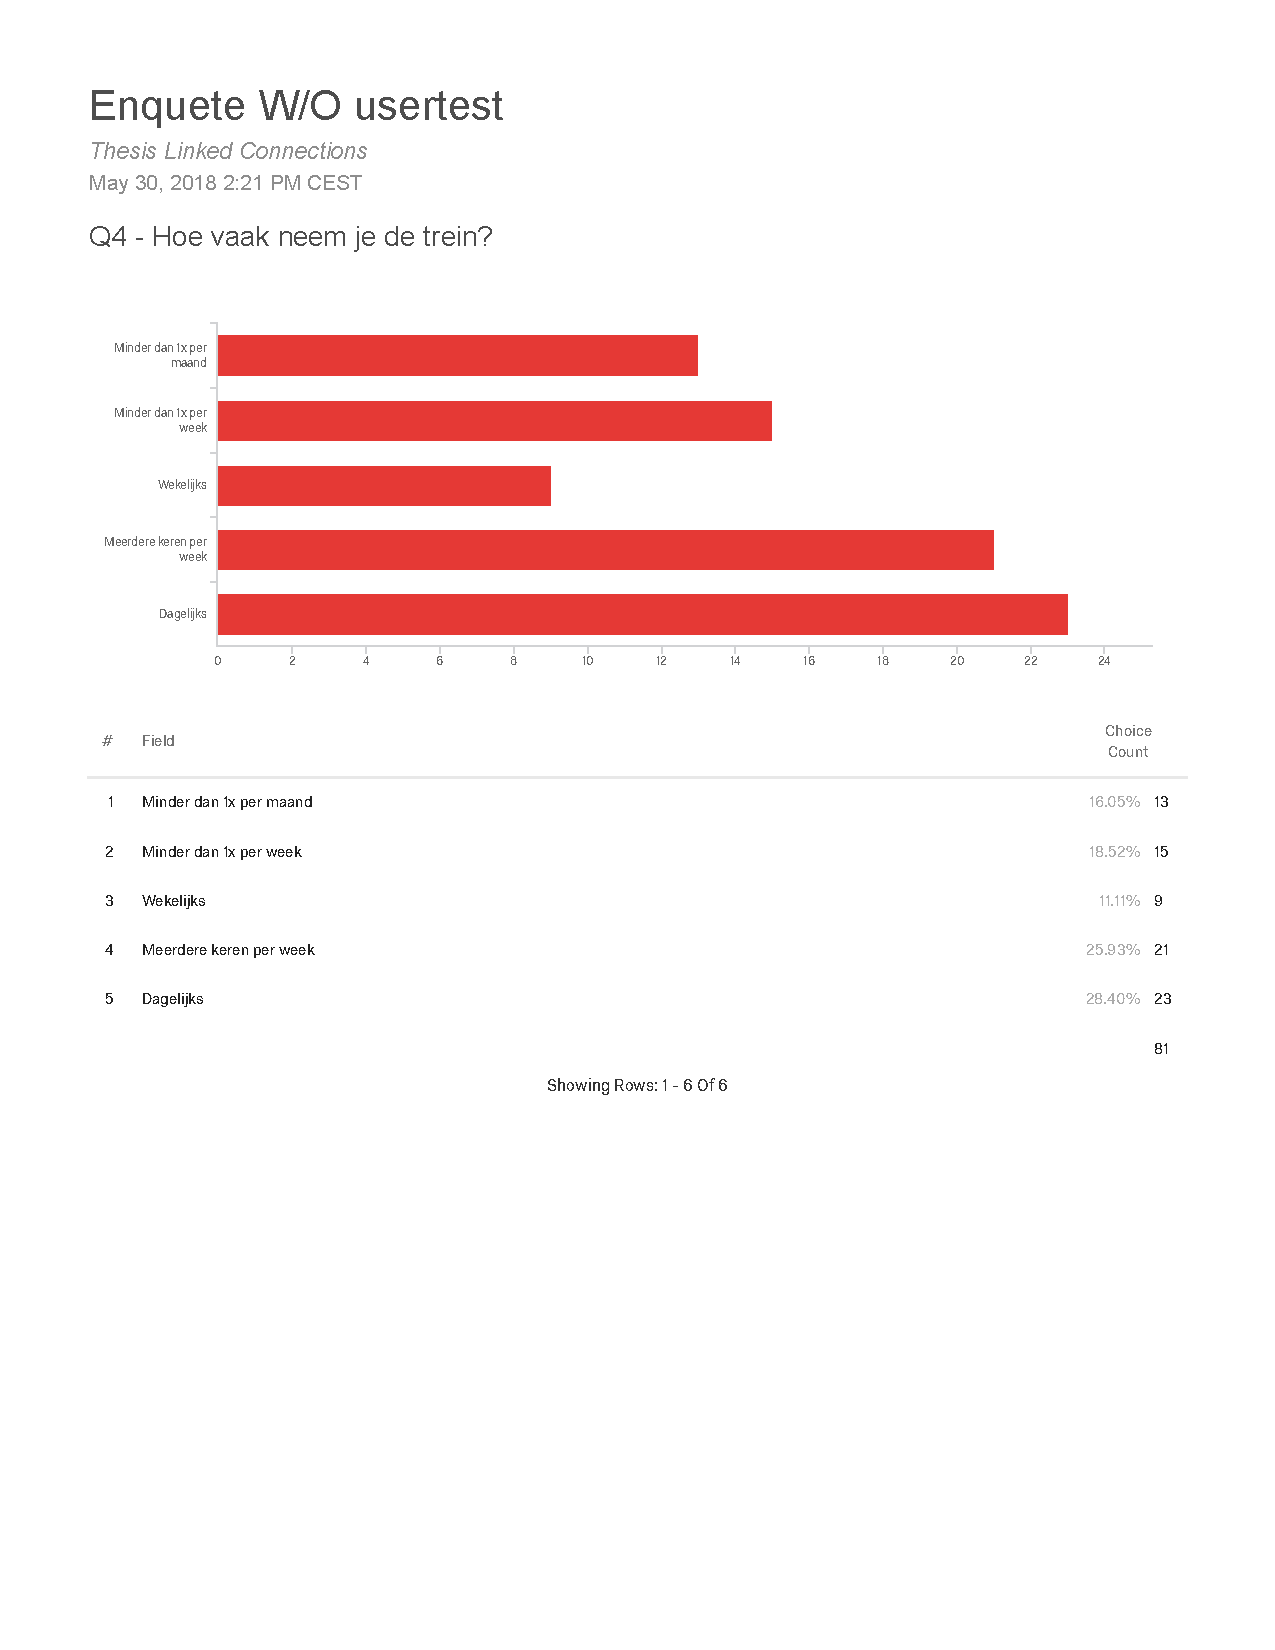
\includepdf[pages=-]{surveyreport.pdf}

\end{appendices}

\end{document}
